\documentclass{beamer}

\usepackage{helvet}
\usepackage{hyperref, graphicx}
\usepackage{amsthm}
\usepackage{etoolbox}

\usetheme{default}
\setbeamertemplate{navigation symbols}{}
\AtBeginSection[ ]
{
\begin{frame}{Outline}
    \tableofcontents[currentsection]
\end{frame}
}

% Default fixed font does not support bold face
\DeclareFixedFont{\ttb}{T1}{txtt}{bx}{n}{12} % for bold
\DeclareFixedFont{\ttm}{T1}{txtt}{m}{n}{12}  % for normal

% Custom colors
\usepackage{color}
\definecolor{TUGray}{RGB}{101,101,137}
\definecolor{TUBlack}{RGB}{30,0,0}
\definecolor{mygreen}{RGB}{45,111,63}
\definecolor{keywords}{RGB}{205,114,0}
\definecolor{comments}{RGB}{181,51,139}
\definecolor{strings}{RGB}{58,144,81}
\definecolor{numeric}{RGB}{66,110,176}
\definecolor{linos}{rgb}{0.4,0.4,0.4}
\definecolor{links}{rgb}{0,0.4,0.75}

\definecolor{bggray}{RGB}{232, 233, 235}

\usecolortheme[named=mygreen]{structure}
\setbeamercolor{normal text}{fg=TUBlack}\usebeamercolor*{normal text}

\setbeamercolor{codecol}{fg=TUGray!25!black,bg=bggray}

\hypersetup{colorlinks, linkcolor=links, urlcolor=links}

\usepackage[T1]{fontenc}
\usepackage[sfdefault,scaled=.85]{FiraSans}
\usepackage{newtxsf}

\usepackage{listings}

\newtoggle{InString}{}% Keep track of if we are within a string
\togglefalse{InString}% Assume not initally in string

\newcommand\digitstyle{\color{numeric}}
\makeatletter
\newcommand{\ProcessDigit}[1]
{%
  \ifnum\lst@mode=\lst@Pmode\relax%
   {\digitstyle #1}%
  \else
    #1%
  \fi
}
\makeatother

\lstset{literate=%
    {0}{{{\ProcessDigit{0}}}}1
    {1}{{{\ProcessDigit{1}}}}1
    {2}{{{\ProcessDigit{2}}}}1
    {3}{{{\ProcessDigit{3}}}}1
    {4}{{{\ProcessDigit{4}}}}1
    {5}{{{\ProcessDigit{5}}}}1
    {6}{{{\ProcessDigit{6}}}}1
    {7}{{{\ProcessDigit{7}}}}1
    {8}{{{\ProcessDigit{8}}}}1
    {9}{{{\ProcessDigit{9}}}}1
    % {<=}{{\(\leq\)}}1,
    % morestring=[b]",
    % morestring=[b]',
    % morecomment=[l]//,
}

% Python style for highlighting
\newcommand\pythonstyle{\lstset{
language=Python,
basicstyle=\ttfamily\tiny,
numbers=left,
numberstyle=\tiny\color{linos},
morekeywords={self},              % Add keywords here
keywordstyle=\tiny\color{keywords},
commentstyle=\it\tiny\color{comments},    % Custom highlighting style
stringstyle=\tiny\color{strings},
xleftmargin=28pt,
xrightmargin=4pt,
aboveskip=0pt,
belowskip=0pt,
escapeinside={(*@}{@*)},
frame=l,                         % Any extra options here
showstringspaces=false,
keepspaces=true
}}

% Python environment 
\lstnewenvironment{python}[1][]
{
	\pythonstyle
	\lstset{
	#1
	}
}
{}

% wrap the Python environment
\newenvironment{codeblock}
    {\hfill\begin{beamerboxesrounded}[lower=codecol, width=0.8\textwidth]
    \medskip

    }
    { 
    \end{beamerboxesrounded}\hfill
    }

\theoremstyle{example}
\newtheorem{question}{Question}

\newcommand{\ct}[1]{\lstinline[language=Python]!#1!}
\newcommand{\ttt}[1]{\texttt{#1}}
\newcommand{\lsitem}[2]{\ttt{{#1}[}\ct{#2}\ttt{]}}

\author{Chris Cornwell}
\date{Dec 17, 2024}
\title{Introduction to Python}

\begin{document}

\begin{frame}
\titlepage
\end{frame}

\begin{frame}
\frametitle{Outline}
\tableofcontents
\end{frame}

\section{Running Python and Jupyter}

%%%%
\begin{frame}
Working in \href{https://www.python.org/}{Python} throughout the semester. 
\begin{itemize}
	\item[] Often interact with Python through Jupyter notebooks (\texttt{.ipynb} files {--} \emph{IPython notebook}).
\end{itemize}

\pause
Two approaches to run and work with Jupyter notebooks.
\begin{enumerate}
	\item Google's Colaboratory {--} \emph{easiest startup}, done in the cloud, extra effort to interact with other files.
	\item Install and run Python and Jupyter on your computer {--} \emph{installation steps to get started}, can work offline, easy to interact with other files.
\end{enumerate}

\href{https://github.com/cornwell/math371-S25/blob/main/Lectures/README.md}{Instructions} for the two approaches.
\end{frame}

%%%%
\begin{frame}
Jupyter notebooks in a nutshell: Markdown cells and Code cells.
	\begin{itemize}
	 	\item Markdown cells, for text: can use HTML code; syntax shortcuts for formatting \& styling. A \href{https://docs.github.com/en/get-started/writing-on-github/getting-started-with-writing-and-formatting-on-github/basic-writing-and-formatting-syntax}{guide for writing in Markdown}.
	 	\pause
	 	\item Code cells: write lines of Python code. The notebook has a Python kernel (session) running; when you ``Run'' or execute a Code cell, the notebook works in that Python session and displays the output (if any).
	\end{itemize}
	\pause
	\begin{figure}
		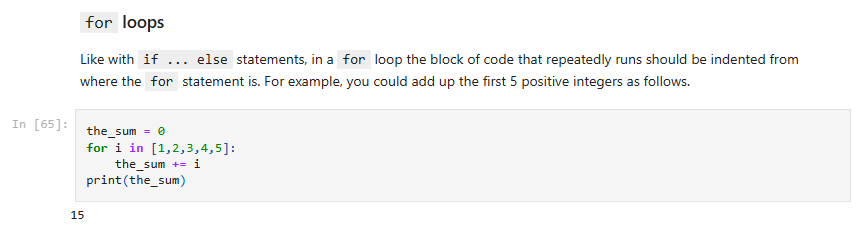
\includegraphics[width=0.7\textwidth]{markdown-code-together.png}
	\caption{{\tiny A Markdown cell followed by a Code cell in a Jupyter notebook}}
	\end{figure}
\end{frame}

\section{Variables and Types}

%%%%
\begin{frame}[fragile]
\frametitle{Assigning variables}

\begin{itemize}
	\item A variable is assigned by placing, on one line, \mbox{\ttt{<variable name> = <assigned value>}.}
\end{itemize}
\begin{codeblock}

\begin{python}
x = 5.11
y = 5
name_full = 'Chris Cornwell'
\end{python}

\end{codeblock}

$\qquad\uparrow$ this code assigns three variables, \ttt{x}, \ttt{y}, and \ttt{name}\ct{_}\ttt{full}

\pause
\begin{itemize}
	\item To ``comment out'' a line, begin line with \#. Good for notes to yourself, or others reading the code.
\end{itemize}

\begin{codeblock}

\begin{python}
# Make an ordered pair; output would be (10.11, 4)
(x + y, y - 1)
\end{python}

\end{codeblock}

\pause
\begin{itemize}
	\item Possible to assign more than one variable in one line.
\end{itemize}

\begin{codeblock}

\begin{python}
x, y = 5.11, 5
# or, you could use 
x = 5.11; y = 5
\end{python}

\end{codeblock}
\end{frame}

%%%%
\begin{frame}[fragile]
\frametitle{Data type}

Each variable has a \emph{data type} (or, simply \emph{type}). 

\begin{codeblock}

\begin{python}
x = 5.11
y = 5
name_full = 'Chris Cornwell'
\end{python}

\end{codeblock}

\begin{itemize}
	\item[] $\uparrow$ the types of the assigned vars are \ct{float}, \ct{int}, and \ct{str} respectively.
\end{itemize}

\pause
Unlike in other programming languages, don't need to declare the types of the variables. Python \emph{interprets} it. (The type might even \emph{change} at a later point.)

\begin{itemize}
	\item type \ct{int}: like an integer.
	\item type \ct{float}: like a real number in decimal form \ldots \emph{kind of}.
	\item type \ct{str}: a ``string,'' or sequence of \emph{characters} (that can be typed from keyboard). Will return to this again.
\end{itemize}
\end{frame}

\section{Operations on different types}

%%%%
\begin{frame}[fragile]
\frametitle{Numerical types}

The four main operations\footnote{Representing addition, subtraction, multiplication, and division.} \ttt{+, -, *,} and \ttt{/} work as you would expect on numerical types \ct{int} and \ct{float}. Unlike when writing math, you cannot leave out \ttt{*} when multiplying.

\pause
\begin{question} Why would it be a \emph{bad} idea to have Python interpret something like \ttt{ab} as being ``\ttt{a} times \ttt{b}''?
\end{question}

\pause

{\bf \color{mygreen} Assigning after an operation.} {\bf Very} often want to change a variable by some amount (e.g., increase it by \ttt{1}); to keep new value, \emph{reassign} after the operation.

\begin{codeblock}

\begin{python}
y = y + 1
# A convenient shorthand for line above is
y += 1
\end{python}

\end{codeblock}

\pause
This is \emph{not} a mathematical equation, but an assignment. The shorthand works for other operations.
\end{frame}

%%%%
\begin{frame}[fragile]
\frametitle{Logical types and {\ttm None}}

We have some logical types, as every language needs {--} \ttt{True} and \ttt{False}. 

Usually, no need to directly assign or work with these. They are ``under the hood'' when making comparisons. 
\pause
\begin{itemize}
	\item Technically, \ttt{True} and \ttt{False} are like \ct{1} and \ct{0} in Python. Use this fact only with \emph{extreme care}! (Maybe just avoid it.)
\end{itemize}
\begin{codeblock}

\begin{python}
(*@ \color{strings}True@*)*(*@\color{strings}False @*)
\end{python}

\end{codeblock}

$\qquad \uparrow$ the line above will return \ct{0}.
\vspace*{12pt}

\pause
The \emph{null} type in Python is {\ttm None}. We'll talk about using it in later lectures.
\end{frame}

\section{Lists}

%%%%
\begin{frame}[fragile]
\frametitle{Basics of lists}

{\ttb list} is a \emph{sequential} data type in Python {--} it holds a sequence of ``items.'' 
\begin{itemize}
	\item[] Each item could be an {\ttb int}, each could be a {\ttb list}, or possibly some with one type, some with another. 
	\pause
	\item[] Example below: a list with {\ttb int} and {\ttb str} type items.
\end{itemize}

\begin{codeblock}

\begin{python}
my_list = [2, 3, 5, 'p']
empty_list = []
\end{python}

\end{codeblock}

\pause
Referring to a list item by index: \\ 
\ttt{my}\ct{_}\lsitem{list}{0} is \ct{2} above, \ttt{my}\ct{_}\lsitem{list}{1} is \ct{3}, and so on.

\pause
The \ttt{+} operation is defined on lists. It results in the \emph{concatenation} of the lists {--} putting them together, end to end.

\begin{codeblock}

\begin{python}
# the code below outputs [2, 3, 5, 'p', 11, 13]
my_list + [11, 13]
\end{python}

\end{codeblock}

\end{frame}

%%%%
\begin{frame}[fragile]
\frametitle{Other operations on lists}

\begin{itemize}
	\item Multiplication by an integer: adds that many copies of the list together. For example, \ct{[1,2]*3} will result in \ct{[1,2,1,2,1,2]}.
	\pause
	\item Length of a list: use the function \ttt{len()}, with your list as input, to get the number of items in your list.
	\pause
	\item Checking if an item is in a list: use the \emph{keyword} \ttt{in} to check this. For example, if \ttt{my}\ct{_}\ttt{list} is \ct{[2, 3, 5, 'p']} then the first line below would result in \ttt{True}, the second would be \ttt{False}.
\end{itemize}

\begin{codeblock}

\begin{python}
print( 2 in my_list )
print( 4 in my_list )
\end{python}

\end{codeblock}

\end{frame}

%%%%
\begin{frame}
\frametitle{Strings and other sequential types}

\begin{itemize}
	\item Some other sequential types: {\ttb tuple}, {\ttb range}.
	\item The operations we discussed (on lists) will work in same way on these.

	\pause
	\item Final important sequential type: {\ttb str}, ``strings.''
	\begin{itemize}
		\item a sequence of \emph{characters}, from your keyboard
	\end{itemize}
	\item Above, the variable that was assigned \ttt{'Chris Cornwell'}, and the item \ttt{'p'} in \ttt{my}\ct{_}\ttt{list}, each is a string.
	\pause
	\item \emph{Thinking} of a string as a list of single characters, operations on strings work like they do on lists (e.g., \ttt{+} will concatenate and \ttt{len()} gives the number of characters, etc. 
\end{itemize}
\end{frame}

%%%%
\begin{frame}[fragile]
\frametitle{{\ttb f}-strings}

To produce output that uses values of some variables in memory: two methods (\emph{there are others I won't mention}).

\pause
Say a variable \ttt{i} is in memory, with \ttt{i = }\ct{2}.

\pause
\begin{codeblock}

\begin{python}
# the next line will print out 'The value of i is 2 .'
print('The value of i is', i, '.')
\end{python}

\end{codeblock}

\begin{itemize}
	\item Works, but has some downsides. 
	\pause
	\item Better: use so-called \ttt{f}-strings, allowing variable(s) directly inside the string, surrounded by braces \ttt{\{ \}}.
\end{itemize}

\begin{codeblock}

\begin{python}
# the next line will print out 'The value of i is 2.'
print(f'The value of i is {i}.')
\end{python}

\end{codeblock}

\pause
\emph{Escape characters} can be handled inside strings also: e.g., \ct{'\\t'} will produce a tab; \ct{'\\n'} produces a newline.

\end{frame}

%%%%
\begin{frame}[fragile]
\frametitle{Two more container types}

Two important types that contain items, but are not sequential are sets ({\ttb set} type) and dictionaries ({\ttb dict} type).
% frame on sets and dictionaries

\begin{itemize}
	\item {\ttb set}: roughly matches the mathematical notion of a set. Items are not ordered; there are no repeated items.
	\pause
	\item {\ttb dict}: has \emph{dictionary keys}; for each key there is an item (the ``entry'' for that key).
	\pause
	\item Two example dictionaries with same keys:
\end{itemize}

\begin{codeblock}

\begin{python}
my_pet = {'name':'Spot', 'age':4, 'type':'dog'}
neighbor_pet = {'name':'Checkers', 'age':2, 'type':'dog'}
\end{python}

\end{codeblock}

\vspace*{12pt}
\pause
Good idea to work with dictionaries for certain kinds of data. Later in the semester, will work with something very similar to a dictionary {--} a DataFrame.
\end{frame}

\section{Intro to Python functions}

%%%%
\begin{frame}[fragile]
\frametitle{Basic functions}

Similar to most programming languages, Python uses \emph{functions}, each of which takes some number of \emph{arguments} (sometimes an argument is optional).

\begin{itemize}
	\item Common function, already encountered: \ttt{print()}.
	\pause
	\item Absolute value: \ttt{abs()}. Takes a numeric argument {--} either {\ttb int} or {\ttb float} type.
	\pause
	\item Round to nearest integer: \ttt{round()}. Takes argument that is {\ttb float} (if an {\ttb int}, will return the same thing).
	\begin{itemize}
		\item Optional 2nd argument, the number of decimal digits.
	\end{itemize}
\end{itemize}
\pause
In Python, run the following to see how \ttt{round()} works.

\begin{codeblock}

\begin{python}
a = -3**2/8
print( a+8 )
print( (round(a+8), round(a+8, 2)) )
\end{python}

\end{codeblock}

\end{frame}

%%%%
\begin{frame}
\frametitle{Changing one type to another}
Some functions change the type of the input, when possible. Some examples:

\begin{itemize}
	\item \ttt{str()} changes to a string; works on nearly anything.
	\pause
	\item \ttt{int()} will convert a float to an int; always rounds toward 0.
	\pause
	\item \ttt{set()} will convert a list or tuple into a set; ``forgets'' order, drops repeats.
\end{itemize}
\end{frame}

%%%%
\begin{frame}[fragile]
\frametitle{Slicing lists}
Recall: if \ttt{my}\ct{_}\ttt{list} is a list, the item at index \ct{i} is found with \ttt{my}\ct{_}\lsitem{list}{i}. 

To get shorter list with consecutive items from \ttt{my}\ct{_}\ttt{list}.

\pause
\begin{codeblock}

\begin{python}
my_list = ['a','b', 'c', 'd', 'e', 'f', 'g', 'h', 'i']
# Return letters at index 1 to 4 (excluding 4)
print(my_list[1:4])

# Leave off number either left of colon, or right of it;
# will go from the start, or until the end
print(my_list[:5])

# Negative numbers to step back from end of the list
print(my_list[-1])
print(my_list[-2:])
\end{python}

\end{codeblock}

\pause
There is an easy way to reverse the order of a list.\footnote{Only as an output. This does not change the list variable unless you reassign it.}

\begin{codeblock}

\begin{python}
my_list[::-1]
\end{python}

\end{codeblock}

\end{frame}

%%%%
\begin{frame}
\frametitle{Basic list methods}

Methods are functions that you call on an instance of a class. There are several methods for lists. Here are two.
\pause
\begin{itemize}
	\item \ttt{append()}: the command \ttt{my}\ct{_}\ttt{list.append(x)}puts \ttt{x} at the end of \ttt{my}\ct{_}\ttt{list}. 
	\begin{itemize}
		\item Changes \ttt{my}\ct{_}\ttt{list} ``in place.''
		\pause
		\item Is equivalent to \ttt{my}\ct{_}\ttt{list += [x]}.
	\end{itemize}
	\pause
	\item \ttt{remove()}: the command \ttt{my}\ct{_}\ttt{list.remove(x)} takes out the \emph{first} item in \ttt{my}\ct{_}\ttt{list} that is equal to \ttt{x}.	
	\begin{itemize}
		\item Changes \ttt{my}\ct{_}\ttt{list} in place, making it shorter.
		\pause
		\item \ttt{my}\ct{_}\ttt{list.pop(i)} does something similar with item at index \ttt{i}, but also returns (has as output) that item.
	\end{itemize}
\end{itemize}

More information on working with lists, tuples, sets, and dictionaries: \href{https://docs.python.org/3/tutorial/datastructures.html}{Tutorial from the Python documentation}.

\end{frame}

\end{document}